\documentclass[a4paper]{article}
\usepackage{graphicx}
\usepackage{float}
\author{Hein van Beers, Jeroen van Hoof}
\title{Automated Reasoning\\
	 \large Practical assignment, Part I}
\begin{document}
	\maketitle
	
	\section{Problem 1}
		\begin{figure}[H]
			\centering
				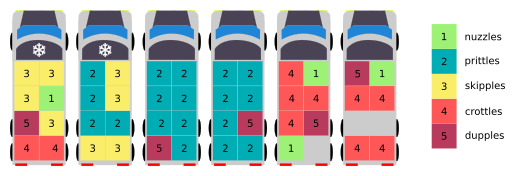
\includegraphics[scale=1]{trucks.png}
			\caption{Placement of pallets on truck. The first two trucks have facility for cooling skipples.}
		\end{figure}
	\section{Problem 2}
	\begin{figure}[H]
		\centering
			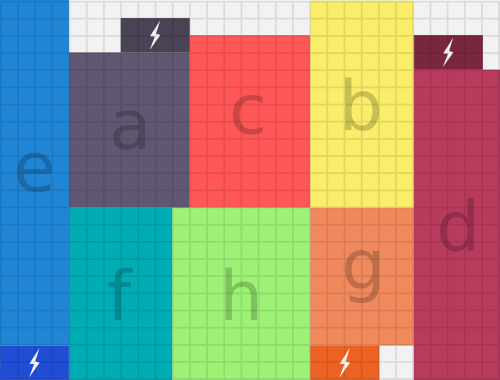
\includegraphics[scale=0.5]{power-grid.png}
		\caption{Placement of components on chip.}
	\end{figure}
	\section{Problem 3}
	\begin{figure}[H]
		\centering
			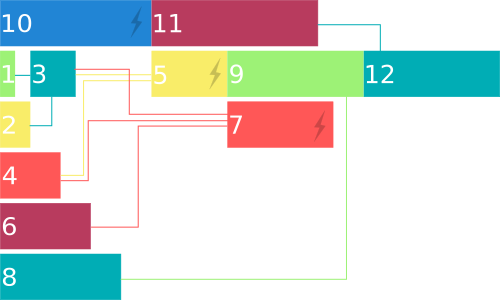
\includegraphics[scale=0.7]{timeline.png}
		\caption{Time-line of process execution. Connected processes depend on each other, special processes are marked with a sign.}
	\end{figure}

\end{document}